\documentclass[11pt]{article}

\usepackage[margin=1in]{geometry}
\usepackage{amsmath,amsthm}
\usepackage{mathtools}
\usepackage{graphicx}
\usepackage{booktabs}
\usepackage{placeins}
\usepackage{dsfont}  % \mathds{1} indicator (OldStandard-Math lacks a bold digit 1)
% Old-style journal look (after tex.stackexchange.com/q/645339): OldStandard text + matching
% OpenType math, small-caps headings, run-in paragraphs. Requires lualatex (pinned in .latexmkrc).
\usepackage{OldStandard}
\usepackage{unicode-math}
\setmathfont{OldStandard-Math.otf}
\usepackage{titlesec}
\usepackage{fancyvrb}
\usepackage[hidelinks]{hyperref}

\linespread{1.15}
\setlength{\parindent}{2em}
\setlength{\emergencystretch}{1em}
\titleformat{\section}{\normalfont\large\scshape\bfseries}{\thesection.}{0.6em}{}
\titleformat{\subsection}{\normalfont\scshape\bfseries}{\thesubsection.}{0.5em}{}
\titleformat{\paragraph}[runin]{\bfseries\scshape}{}{0pt}{}[.]
\titlespacing*{\paragraph}{\parindent}{0.4em}{0.6em}

\newtheoremstyle{oldplain}{}{}{\itshape}{}{\scshape}{.}{.5em}{}
\newtheoremstyle{oldrem}{}{}{\normalfont}{}{\scshape}{.}{.5em}{}
\theoremstyle{oldplain}
\newtheorem{proposition}{Proposition}
\theoremstyle{oldrem}
\newtheorem{definition}{Definition}
\newtheorem{remark}{Remark}

\newcommand{\Pgen}{P_{\mathrm{gen}}}
\newcommand{\ins}{\mathrm{ins}}
\newcommand{\del}{\mathrm{del}}
\newcommand{\indic}{\mathds{1}}

\title{\scshape The V(D)J rearrangement model and exact generation probabilities in \texttt{vdjtools}}
\author{Mikhail Shugay\textsuperscript{1,2,3}\thanks{Correspondence:
  \href{mailto:mikhail.shugay@gmail.com}{mikhail.shugay@gmail.com}}}
\date{%
  \small
  \textsuperscript{1}Institute of Translational Medicine, Russian National Medical State University, Moscow, Russia\\
  \textsuperscript{2}Department of Genomics of Adaptive Immunity, Shemyakin--Ovchinnikov Institute of Bioorganic Chemistry RAS, Moscow, Russia\\
  \textsuperscript{3}Institute of Molecular Biology NAS RA, Yerevan, Armenia\\[6pt]
  \normalsize\textit{Appendix M --- \texttt{vdjtools} model engine}%
}

\renewcommand{\thesection}{M.\arabic{section}}

\begin{document}
\maketitle

\begin{abstract}
\noindent
The \texttt{vdjtools} model engine implements the Murugan--Marcou generative model of V(D)J
recombination \cite{Murugan2012,Marcou2018} on the AIRR schema \cite{VanderHeiden2018}, storing every
model factor as a tidy \texttt{polars} table so that the Bayesian-network structure is declared as data
rather than hidden in an opaque file format. On top of this representation it computes the generation
probability ($\Pgen$) of a junction --- the total probability that the stochastic recombination process
produces a given sequence --- both for nucleotide queries (an exact scenario sum) and, more delicately,
for amino-acid queries, where one must marginalise over all synonymous nucleotide realisations. For the
amino-acid case we use the transfer-matrix factorisation of \cite{Sethna2019}, but re-derive
it from a single structural observation --- \emph{that the only coupling across a recombination-block
boundary is codon translation, never the insertion Markov chain} --- which yields a clean left/right
partial-sum split (\S\ref{sec:aa}) that our native C++ core evaluates with machine-precision agreement to \texttt{OLGA} on identical legacy parameters
(\S\ref{sec:bench}). The same tables and scenario enumeration
drive sequence generation (ancestral sampling) and model inference (expectation--maximisation), which we
describe in \S\ref{sec:em}.
\end{abstract}

\paragraph{Scope and terminology} This appendix describes the current
\texttt{vdjtools} model engine and distinguishes its working \texttt{isalgo} models from frozen
\texttt{olga-legacy} parameters.
An AIRR \emph{junction} includes the conserved Cys104 and Phe/Trp118 codons;
the IMGT CDR3 excludes these anchors.
The historical OLGA API calls this anchor-inclusive sequence a CDR3.
All sequence lengths, coordinates and probabilities below refer to the junction.
The notation first introduces the single-$D$ factorisation, then extends it to the
joint single/tandem histories used by current VDJ fits.
The reference principles are the latent-history likelihood of Murugan et al.,
including its Supporting Information, and IGoR's probabilistic scenario search
\cite{Murugan2012,Marcou2018}; the insertion boundary convention here is stated explicitly below.

\section{The generative recombination model}\label{sec:model}

A rearranged receptor chain is the output of a stochastic process that (i) selects germline segments,
(ii) trims their ends by exonuclease deletion, and (iii) inserts non-templated nucleotides at the
junctions. Following \cite{Murugan2012,Marcou2018} we treat a \emph{recombination scenario} $r$ --- the
full list of hidden events --- as a sample from a Bayesian network whose factors are the model
parameters. For a $VDJ$ locus (TRB, TRD, IGH) a scenario is
\begin{equation}\label{eq:scenario}
  r=\bigl(V,\,J,\,D,\;\del_V,\,\del_J,\,\del_D^{5'},\,\del_D^{3'},\;\mathbf{m}^{VD},\,\mathbf{m}^{DJ}\bigr),
\end{equation}
with probability
\begin{equation}\label{eq:pvdj}
  P(r)=P(V)\,P(J)\,P(D\mid J)\;
       P(\del_V\!\mid V)\,P(\del_J\!\mid J)\,P(\del_D^{5'},\del_D^{3'}\!\mid D)\;
       P_{\ins}(\mathbf{m}^{VD})\,P_{\ins}(\mathbf{m}^{DJ}).
\end{equation}
A $VJ$ locus (TRA, TRG, IGK, IGL) has no $D$ segment; its scenario drops $D$, the two $D$-deletions and
one insertion, and the gene factor becomes the joint $P(V)\,P(J\mid V)$ with a single $VJ$ insertion.
The generated junction nucleotide sequence $\sigma(r)$ is the concatenation, from the conserved Cys\,104 to
the conserved Phe/Trp\,118 inclusive,
\begin{equation}\label{eq:concat}
  \sigma(r)=\underbrace{\hat V}_{\text{V germline}}\;
            \underbrace{\mathbf{m}^{VD}}_{\text{N1}}\;
            \underbrace{\hat D}_{\text{D germline}}\;
            \underbrace{\mathbf{m}^{DJ}}_{\text{N2}}\;
            \underbrace{\hat J}_{\text{J germline}},
\end{equation}
where $\hat V,\hat D,\hat J$ are the germline segments after the indicated deletions.

\paragraph{Insertion chains} Each non-templated segment $\mathbf{m}=m_1\cdots m_\ell$ is drawn from a
length distribution and a first-order Markov chain:
\begin{equation}\label{eq:ins}
  P_{\ins}(\mathbf{m}) = P_{\ins}(\ell)\; b(m_1)\prod_{i=2}^{\ell} R(m_i\mid m_{i-1}),
\end{equation}
with $b$ the first-nucleotide distribution and $R$ the $4\times4$ transition matrix.
For zero insertion length, only the length factor contributes. New scaffolds fit
$b$ independently, counting the first base of every nonempty insertion, including
length-one insertions with no transition. Unobserved transition conditionals
retain their normalised initial rows; zeroing them would lose probability mass
when first bases and insertion lengths recombine independently. Models without
explicit first-base events retain the legacy stationary-$R$ convention.
The $VD$ chain is read $5'\!\to\!3'$ and the $DJ$ chain $3'\!\to\!5'$, so $b_{DJ}$
describes the $J$-proximal insertion nucleotide. This independent first-base
distribution differs from IGoR's first transition conditioned on the adjacent
retained germline nucleotide. In table form, \texttt{from\_nt,to\_nt,p} stores
$R(b\mid a)$ with $a$ the previous nucleotide and $b$ the next; the packed native
array uses the equivalent column-stochastic convention $R[b,a]$.

\paragraph{Generation probability} The quantity of interest is the probability of a specified
junction, obtained by summing over every scenario that could have produced it,
\begin{equation}\label{eq:pgen}
  \Pgen(\sigma) \;=\; \sum_{r\,:\,\sigma(r)=\sigma} P(r),
  \qquad
  \Pgen(\alpha) \;=\; \sum_{\sigma\,:\,\tau(\sigma)=\alpha}\Pgen(\sigma),
\end{equation}
where $\tau$ is translation: an amino-acid query $\alpha$ additionally marginalises over all synonymous
nucleotide sequences. Both sums are finite but astronomically large if taken literally; \S\ref{sec:nt}
and \S\ref{sec:aa} evaluate them by dynamic programming.

\section{Model parameters as data}\label{sec:tables}

\texttt{vdjtools} stores a model as a directory of long-format \texttt{polars} parquet tables plus a
\texttt{manifest.json} that names each event and lists its conditioning parents --- the edges of the
Bayesian network of Eq.~\eqref{eq:pvdj}. The engine implements the declared supported
factorisations; changing parents alone does not implement a richer dependency
such as $P(D\mid V,J)$, which also requires compatible packing, inference and
sampling. A $VJ$ locus omits the $D$ tables and second insertion. Each table holds the
distribution of one event, normalised within its conditioning key by a single \texttt{polars}
\texttt{group\_by} --- which is exactly the M-step of \S\ref{sec:em}. Two conventions matter for the
$\Pgen$ recursions.

\paragraph{P-nucleotides} A negative deletion count encodes templated palindromic (P-)
nucleotides. Each germline cut segment is pre-extended by up to \texttt{maxpal} reverse-complement
nucleotides; a ``deletion'' of $-k$ means $k$ P-nucleotides are retained. The stored count $\del$ is thus
\emph{biological} (negative $=$ P-nucleotides), while the dense array index used at run time is
$\del+\texttt{maxpal}\ge 0$.

\paragraph{Germline references and gene resolution} Native scaffolds resolve V/D/J
sequences and anchor coordinates from \texttt{arda}.
V germline is cut from its anchor to its 3$'$ end; J germline extends from its
5$'$ end through the anchor codon.
Anchor offsets are zero-based nucleotide coordinates in each full reference, not
codon indices; references can differ in framework length or sequence even when
these conventions agree.
A model never mixes germline sources: models imported from \texttt{OLGA} retain
their imported reference, whereas native fits use \texttt{arda}.
Raw-OLGA engine comparisons explicitly disable anchor repairs so both engines
receive identical germline sequences.
New native models select one usable, complete, functional major allele per gene:
\texttt{*01} when available, otherwise the lowest-numbered usable allele.
Allele suffix aliases resolve to this representative without adding probability
mass; ambiguity between different genes remains in the scenario sum.
Explicit all-allele models retain allele-specific templates and scoring.
Unknown calls raise rather than silently becoming unrestricted gene sums.

\paragraph{The D-D extension} The schema carries single- and tandem-$D$
rearrangements, including a second-$D$ deletion and a $DD$ insertion, beyond the
single-$D$ event graphs used here as \texttt{OLGA}/IGoR references
(\S\ref{sec:dd}). The current joint-history models use $n_D\in\{1,2\}$; a fully deleted
single D remains a one-D latent history, even though it contributes zero retained
nucleotides. A strict single-D model has no tandem history by construction.

\section{Nucleotide generation probability}\label{sec:nt}

For a nucleotide query $\sigma$ the inner sum of Eq.~\eqref{eq:pgen} is a direct enumeration, because each candidate germline placement fixes the remaining insertion strings. Writing $N=|\sigma|$ and letting a $V$
(resp.\ $J$) contribute $\ell_V\ge1$ (resp.\ $\ell_J\ge1$) nucleotides --- a valid rearrangement is never
fully $V$- or $J$-deleted, matching \texttt{OLGA} ---
\begin{equation}\label{eq:pgennt}
  \Pgen(\sigma)=\!\!\sum_{V,J}\! G(V,J)\!\!
    \sum_{\substack{\ell_V,\ell_J\ge 1,\ \ell_V+\ell_J\le N\\ \sigma[0{:}\ell_V]=\hat V,\ \sigma[N-\ell_J{:}]=\hat J}}
    \!\! P(\del_V\mid V)P(\del_J\mid J)\;\Xi_J\bigl(\sigma[\ell_V{:}N-\ell_J]\bigr),
\end{equation}
where $G(V,J)=P(V)P(J\mid V)$ for VJ and $G(V,J)=P(V)P(J)$ for VDJ.
For a $VJ$ locus $\Xi_J(\mu)=P_{\ins}(\mu)$ is the single-junction insertion weight of
Eq.~\eqref{eq:ins}, and for a $VDJ$ locus $\Xi_J$ is itself a sum over the $D$ gene, its two deletions and
its placement,
\begin{equation}\label{eq:dmiddle}
  \Xi_J(\mu)=\sum_D P(D\!\mid\! J)\!\!\sum_{\del_D^{5'},\del_D^{3'}}\!\! P(\del_D^{5'},\del_D^{3'}\mid D)
    \sum_{\substack{\text{placements }p\\ \mu[p{:}p+\ell_D]=\hat D}}\!\!
    P_{\ins}\bigl(\mu[0{:}p]\bigr)\,P_{\ins}\bigl(\mu[p+\ell_D{:}]\bigr).
\end{equation}
Common-prefix / common-suffix matching restricts $\ell_V,\ell_J$ to the genes that can actually flank
$\sigma$, so Eq.~\eqref{eq:pgennt} is fast in practice. This exact nucleotide sum supplies the zero-error E-step; the observation-error
channel modifies its germline emission factors (\S\ref{sec:em}). On identical raw legacy parameters, the native port reproduces \texttt{OLGA}'s \texttt{compute\_nt\_CDR3\_pgen} to
machine precision.

\section{Tandem-D (D-D) rearrangements}\label{sec:dd}

A tandem-$D$ locus joins two $D$ segments in the junction,
$V\!-\!D_1\!-\!D_2\!-\!J$. New joint-history models store
\begin{equation}\label{eq:dhistory}
 q_J(n,D_1,D_2)=P(n,D_1,D_2\mid J),\qquad
 \sum_{(n,D_1,D_2)\in\mathcal S_J}q_J(n,D_1,D_2)=1.
\end{equation}
Here $\mathcal S_J$ contains physically permitted histories, $n\in\{1,2\}$,
and $D_2$ is absent for $n=1$. Thus the single-$D$ probability can vary with $J$;
there is no independent global $P(n_D)$ factor in this representation.
TRB permits $D_1$--$D_2$--$J_2$ and single $D_1$--$J_2$ histories.
Human TRD histories follow the curated forward coding order
TRDD1--TRDD2--TRDD3. Constraints act on complete histories before fitting,
not on fitted probability tables afterwards.
The implemented extension retains at most two D genes; it does not enumerate
three-D histories. No universal 10\% tandem-D ceiling is imposed.
A preliminary greedy alignment cannot veto a permitted history.

A two-$D$ scenario has probability
\begin{equation}\label{eq:pdd}
 \begin{aligned}
 P(r_2)={}&P(V)P(J)q_J(2,D_1,D_2)P(\del_V\mid V)P(\del_J\mid J)\\
 &{}\times P(\del_{D_1}\mid D_1,n=2)P(\del_{D_2}\mid D_2,n=2)
 \prod_{u\in\{VD,DD,DJ\}}P_{\ins}(\mathbf m^u).
 \end{aligned}
\end{equation}
Its junction is $\sigma(r_2)=\hat V\,\mathbf m^{VD}\,\hat D_1\,
\mathbf m^{DD}\,\hat D_2\,\mathbf m^{DJ}\,\hat J$.
For $n=1$, use $q_J(1,D_1,\varnothing)$, its separate single-$D$ deletion
conditional, and omit the $D_2$ and $DD$ factors. Consequently
\begin{equation}\label{eq:ximix}
 \Xi_J(\mu)=\sum_{r:\,\sigma_{\mathrm{middle}}(r)=\mu}
 q_J(n,D_1,D_2)P(\text{middle trims and insertions}\mid n,D_1,D_2).
\end{equation}

\begin{proposition}[Disjoint latent histories]\label{prop:dd}
Both retained $D$ segments in a tandem history have at least one nucleotide.
Single-$D$ histories allow complete $D$ deletion. These are disjoint sets of
latent histories, but their emitted nucleotide sequences can overlap.
Their mixture is normalised when $q_J$ and every reachable conditional are normalised.
\end{proposition}

Requiring nonempty tandem segments is an explicit model convention; it does not
make the number of $D$ segments identifiable from a sequence. In particular,
insertions can coincidentally match germline bases. The inference and generation
kernels use separate normalised single-$D$, tandem-first-$D$ and second-$D$
deletion tables, so removing fully deleted tandem states does not leak probability.
EM accumulates posterior counts directly over $\mathcal S_J$, then normalizes within
$J$. An optional single-$D$ pseudocount is divided uniformly among declared
single-$D$ history rows within each $J$. Undefined groups retain their initial
normalised conditional. The reported $D$-count probability is
$P(n)=\sum_JP(J)\sum_{D_1,D_2}q_J(n,D_1,D_2)$.

Native and reference nucleotide/amino-acid Pgen, generation and E-step kernels
use these same factors. The native codon-constrained max-product search also
includes tandem paths and reconstructs both $D$ spans. Legacy models retain their
existing global $P(n_D)P(D_1\mid J)P(D_2\mid D_1)$ representation and artefact behavior;
the joint-history schema is an explicit conversion, not a reinterpretation of
frozen tables.

\section{Amino-acid generation probability by transfer matrix}\label{sec:aa}

The amino-acid case is harder: the codon marginalization in Eq.~\eqref{eq:pgen} reintroduces a sum over
the unobserved junction nucleotides. Enumerating scenarios and summing synonymous codons position by
position (a codon-constrained dynamic program of width $|\Sigma|$ over the nucleotide state) is correct
but costs one $O(N)$ pass per $(D,\del_D^{5'},\del_D^{3'},\text{placement})$ skeleton --- quadratic in
$N$ and prohibitive for long junctions. The transfer-matrix method reuses partial sums across placements and insertion lengths.

\paragraph{Setup} Let $\alpha=\alpha_0\cdots\alpha_{L-1}$ be the query, $N=3L$, and $\sigma_i$ the (summed
over) nucleotide at position $i$. Codon $c$ imposes
$\tau(\sigma_{3c},\sigma_{3c+1},\sigma_{3c+2})=\alpha_c$. Because the codon and the insertion Markov chain
each look back at most two and one nucleotide respectively, a left-to-right dynamic program with state
$x_i=(\sigma_{i-1},\sigma_{i-2})$ suffices: it can (a) close a codon when $i\equiv 2\pmod 3$ and (b) carry
the Markov dependency. The width is $|\Sigma|=25$ (four nucleotides plus a start sentinel, squared). This
is the codon-marginalizing DP; the transfer matrix is what lets us reuse its partial results across all
scenarios.

\paragraph{The key structural fact} In the block layout of Eq.~\eqref{eq:concat},
$\hat V$--$\mathbf{m}^{VD}$--$\hat D$--$\mathbf{m}^{DJ}$--$\hat J$, the blocks are coupled only through
codon translation, never through an insertion Markov chain.

\begin{proposition}[Codon-only coupling]\label{prop:coupling}
For fixed gene choices and trimming events, the nucleotide-dependent weight
across each block boundary in Eq.~\eqref{eq:concat} factors into a left
factor, the indicator(s) of the codon(s) straddling the boundary, and a right factor. No transition
$R(\cdot\mid\cdot)$ spans a boundary.
\end{proposition}
\begin{proof}[Sketch]
The $VD$ chain's leftmost nucleotide $m^{VD}_1$ is drawn from the bias $b_{VD}$ independent of the last
$V$ nucleotide, and its rightmost nucleotide carries no transition into $\hat D$; the $D$ block is
germline (fixed nucleotides, no chain); the $DJ$ chain, read $3'\!\to\!5'$, draws its $J$-proximal
nucleotide from $b_{DJ}$ independent of the first $J$ nucleotide, and its $D$-proximal nucleotide carries
no transition into $\hat D$. Hence every factor in Eq.~\eqref{eq:ins} lives strictly inside one block.
The only inter-block constraints are the codon indicators $\indic[\tau(\cdots)=\alpha_c]$ for codons that
straddle a boundary.
\end{proof}

Proposition~\ref{prop:coupling} licenses computing the left and right halves of the sum \emph{once each}
and stitching them, instead of recomputing a full pass per scenario.

\paragraph{Left partial sums} Define, for each boundary position $p$ (the position at which $\hat D$
starts) and each nucleotide state $x=(\sigma_{p-1},\sigma_{p-2})$,
\begin{equation}\label{eq:lambda}
  \Lambda_p(x)=\!\!\sum_{\substack{V,\,\del_V,\,\ell_{VD}\\ \ell_V+\ell_{VD}=p}}\!\!
    P(V)P(\del_V\mid V)\,P_{\ins}(\ell_{VD})\;\bigl[\text{$VD$ Markov}\bigr]\;
    \prod_{\text{codons }\subset[0,p)}\!\!\indic[\tau=\alpha],
\end{equation}
the total weight of all ways the $V$ germline (with $\ell_V\ge1$) plus the $VD$ insertion fill
$[0,p)$ ending in state $x$, with every codon that lies wholly in $[0,p)$ satisfied. $\Lambda$ is built
by one forward recursion: germline seeds are deposited at $p=\ell_V$, then the $VD$ transfer step
--- multiply by $b_{VD}$ on the first inserted nucleotide and $R_{VD}$ thereafter, close codons at
$p-1\equiv2\pmod3$, and add $P_{\ins}(\ell_{VD})$ at each length --- extends them, in $O(NK_{VD}|\Sigma|)$ work after seeding, where $K_{VD}$ is the
maximum supported VD insertion length, truncated to $N$.
The code starts a separate insertion recursion from each supported germline
boundary; it is quadratic in $N$ when $K_{VD}$ grows with $N$.

For a seed boundary $q$, let $W_{q,0}$ be its germline-seeded state vector,
including gene and deletion weights. For $\ell\ge1$, the forward update is
\begin{equation}\label{eq:forward}
 W_{q,\ell}(a,b)=\sum_{c}W_{q,\ell-1}(b,c)\,
 \begin{cases}b_{VD}(a),&\ell=1,\\R_{VD}(a\mid b),&\ell>1\end{cases}
 \chi_{q+\ell-1}(c,b,a),
\end{equation}
where $a,b,c$ are nucleotide states and $\chi_i$ is one unless $i\equiv2\pmod3$;
in that phase it tests the completed codon against the query.
Unavailable leading bases are represented by the sentinel and never enter a
completed codon test.
Then $\Lambda_p=\sum_{q+\ell=p}P_{\ins}(\ell)W_{q,\ell}$, including $\ell=0$.
Insertion length weights enter this sum, not the propagation from $\ell$ to $\ell+1$.

\paragraph{Right partial sums} Symmetrically, for each $D$ gene and boundary $p$ (where $\hat D$ ends),
\begin{equation}\label{eq:rho}
  \Psi^D_p(y)=\!\!\sum_{J,\,\del_J,\,\ell_{DJ}}\!\!
    P(D\!\mid\! J)P(J)P(\del_J\mid J)\,P_{\ins}(\ell_{DJ})\;\bigl[\text{$DJ$ Markov}\bigr]\;
    \prod_{\text{codons }\subset[p,N)}\!\!\indic[\tau=\alpha],
\end{equation}
with $y=(\sigma_p,\sigma_{p+1})$ and
$p+\ell_{DJ}+\ell_J=N$ in the sum. Because the $DJ$ chain runs $3'\!\to\!5'$, $\Psi^D$ is built by a
\emph{backward} recursion from the $J$ boundary --- one per $D$ gene, the $P(D\mid J)$ weight folded into
the seed. There are at most $d$ such passes, where $d$ is the number of D templates,
each costing $O(NK_{DJ}|\Sigma|)$ after seeding.
This $d$ is distinct from the latent D-count event $n_D$.

\paragraph{Stitching} Fixing $D$, its deletions (hence the fixed germline string $\hat D$ of length
$\ell_D$) and its start $p_0$, thread the germline nucleotides of $\hat D$ through the DP from $\Lambda_{p_0}$
to a state distribution at $p_1=p_0+\ell_D$ (closing any codons interior to $\hat D$, no Markov weight),
then contract with $\Psi^D_{p_1}$. By Proposition~\ref{prop:coupling} at most one codon straddles the
$D/DJ$ boundary $p_1$; the contraction is a bounded codon-state contraction (or scalar product when $p_1\equiv0\pmod3$) over that
codon's free nucleotides. Summing over $D$, its deletions and $p_0$,
\begin{equation}\label{eq:stitch}
  \Pgen(\alpha)=\sum_D\ \sum_{\del_D^{5'},\del_D^{3'}} P(\del_D^{5'},\del_D^{3'}\mid D)
    \sum_{p_0}\ \Bigl\langle\, \mathcal{T}_{\hat D}\,\Lambda_{p_0}\,,\ \Psi^D_{p_1}\,\Bigr\rangle_{p_1},
\end{equation}
where $\mathcal{T}_{\hat D}$ is the germline-threading operator and $\langle\cdot,\cdot\rangle_{p_1}$ the
codon-contracting stitch at $p_1$. The insertion-length sums are already inside $\Lambda$ and $\Psi^D$, so
the outer work is $O\!\bigl(d\cdot\#\!\del_D\cdot N\cdot\ell_D\bigr)$ with $\ell_D\ll N$ --- versus the
enumeration's extra factor of $N$ from re-running the DP per placement. For a $VJ$ locus there is no $D$
and no D bridge: for each retained J template, the code builds a left DP with
$P(J\mid V)$ in the V seed and threads each supported J suffix into its boundary state.
The resulting computation still sums all supported V/J trims and insertion lengths.

\begin{remark}
This is the $\Pi_L\!\cdot\!\Pi_R$ factorisation of \cite{Sethna2019} expressed on the
\texttt{polars} tables. Where \texttt{OLGA} handles the $D$ block with a sliding right-deletion recursion
folded into $\Pi_R$, we keep $\Psi^D$ purely $J$/$DJ$ and slide a short explicit germline bridge
(Eq.~\eqref{eq:stitch}); the two agree to machine precision (\S\ref{sec:bench}), and the explicit bridge
is what generalizes to the tandem-$D$ event.
\end{remark}

\paragraph{Exact tandem contraction}
Let $N$ be the junction nucleotide length, $S=25$ the codon-state count,
$D$ the number of functional D templates, and $J$ the number of selected J
alleles. The native engine builds the V/VD left matrix once.
For each first D template $d$, it sums all supported nonempty retained-D
histories ending at each boundary/state and extends that sum through the DD
insertion recurrence. Call the resulting matrix $M_d$.
This matrix contains the first-D deletion weight but no J-dependent history
weight. For each J allele $j$, $R_j$ contains $P(J=j)$, J trimming and DJ
insertion factors. Let $H_{jde}$ denote the joint tandem-history weight for
first D $d$ and second D $e$, or the legacy product
$P(d\mid j)P(e\mid d)$. Forbidden complete histories have $H_{jde}=0$.

For fixed second D $e$, let $C_e(A,B)$ mean threading every supported nonempty
trim of $e$ through left message $A$, multiplying by its second-D deletion
probability, and stitching with right message $B$ using
Eq.~\eqref{eq:stitch}. This operation is bilinear, so the tandem branch is
\begin{align}
 T &= \sum_{d,e} C_e\!\left(M_d,\sum_j H_{jde}R_j\right)
    = \sum_{j,e} C_e\!\left(\sum_d H_{jde}M_d,R_j\right).
\end{align}
The global tandem-mixture weight, when present, multiplies $T$ exactly once
in the caller. The implementation chooses between these expressions using the active first-D
and J counts, after removing complete histories with exactly zero weight or
forbidden support. The second-D templates remain unrestricted by that choice. Thus it performs at most
$\min(D^2,JD)$ second-D bridge walks, rather than $JD^2$, and computes each
$M_d$ only once. Mixing messages costs $O(JD^2NS)$ in the dense worst case;
zero history weights are skipped. Message storage is $O((J+D)NS)$ in the
second form and $O(JNS)$ in the first, excluding the existing fixed-size
codon-state scratch.

Both D roles share a prefix walk over placements and 5-prime trims. Successive
retained lengths extend the same prefix instead of rethreading each 3-prime
trim from its beginning. A zero codon-compatible message terminates every
longer prefix exactly. After two fixed bases, the message has only one possible
codon state, so subsequent fixed bases use a scalar state transition.
The first- and second-base messages are shared across 5-prime cuts for each
input matrix. At a DD-insertion end, completed codons can be forgotten before
the fixed second-D block: boundary phases zero, one and two need respectively
zero, one and two past bases. Thus at most 1, 4 or 16 canonical states remain,
further restricted by the codon mask. Only those cells enter the D-pair mixing
loop. Inside the DD insertion, the last inserted base remains necessary for the
Markov transition even when a codon has just ended. The exact interior state
counts at phases zero, one and two are therefore 4, 4 and 16. Let $x_q^{(0)}(a)$
and $x_q^{(1)}(a)$ denote masses at nucleotide boundary $q$ with last base $a$,
and let $x_q^{(2)}(a,b)$ retain the two most recent bases, newest first.
With $R_{ca}=P(c\mid a)$, the subsequent insertion steps are
\begin{align}
 x_{q+1}^{(1)}(c) &= \sum_a x_q^{(0)}(a)R_{ca}, &&q\equiv0\pmod3,\\
 x_{q+1}^{(2)}(c,a) &= x_q^{(1)}(a)R_{ca}, &&q\equiv1\pmod3,\\
 x_{q+1}^{(0)}(c) &= \sum_{a,b}x_q^{(2)}(a,b)R_{ca}
       \mathbf{1}\{(b,a,c)\in A_{\lfloor q/3\rfloor}\}, &&q\equiv2\pmod3.
\end{align}
Here $A_k$ is the allowed codon set at amino-acid position $k$. The first inserted
base uses its fitted first-base bias rather than a transition from the preceding
germline. Zero insertion uses the original seed directly. Each supported
insertion length multiplies its endpoint mass exactly once. At insertion end,
the states project back to the 1/4/16 canonical fixed-D boundary representation.
The aggregation forgets only bases absent from both the unfinished codon and the
next Markov transition, so it preserves the complete nonnegative history sum.
It reduces state work without truncating insertion-length support.
First-/two-base preparation is shared across D templates only when their incoming
matrix is identical. In the left-mixing contraction the input differs for each
$(j,e)$ and is prepared separately. Exact AA batches own bounded prefix scratch
per worker and reset active entries for every new input; selected batches use
one immutable model with small J-dependent V-choice arrays. No computed Pgen
result is cached between calls or queries.

All nonzero deletion weights remain; a prefix shorter than the first supported
length still propagates because it can lead to a longer supported fragment.
Each D retains at least one nucleotide and J retains at least one nucleotide.
No minimum retained-D length beyond this model convention, probability cutoff,
or renormalization is used. Linearity proves equivalence in exact arithmetic;
changing nonnegative reduction order can change floating-point rounding.
Native singleton-codon NT masks, AA masks, degenerate masks and Hamming-1 calls
use this same kernel. The V+VD message is computed once and shared across
single-D and tandem branches of the mixture; single-D coefficients and frozen
OLGA probabilities retain their original meanings.

For each right message, the boundary join has an adjoint coefficient vector
$B_j(q,s)$ such that $\operatorname{join}(A,R_j;q)=\sum_s A(q,s)B_j(q,s)$.
It is computed once per right message and reused over all second-D trims.
After two fixed D bases only one left state survives, so each terminal join
becomes one multiplication. This is the same nonnegative bilinear form;
no retained-prefix contribution is omitted.

For a nonnegative sum of $k$ fixed floating-point terms, sequential accumulation
has relative rounding-error bound $\gamma_k=ku/(1-ku)$ when $ku<1$, where
$u$ is unit roundoff. This bound concerns the sum alone, not errors already
present in its terms. A contraction with fewer additions can therefore be more
accurate than the original enumeration while differing from its double result.
In the Linux 1,000-query IGH comparison, 32 differences exceeded $10^{-12}$
relative to the old double accumulation. Re-evaluating all 32 with the original
kernel and only its final tandem accumulator promoted to long double gave
maximum relative errors $4.8\times10^{-13}$ for the optimized contraction and
$5.9\times10^{-12}$ for the original double result. No probability cutoff was
introduced to obtain this agreement.

\section{Optional coarse post-selection calibration}

The recombination model and its error-free generation probabilities remain
unchanged. The optional selection model retains a joint V/J factor and a shared
length factor from the factorized approach of Elhanati et al.\ \cite{Elhanati2014},
without amino-acid-position factors. Here $L$ counts amino acids including the
conserved C and terminal F/W. Let $g=(v,j)$ be a gene pair and let
$P_0(g,L)$ be the exact recombination mass conditioned on a C-first,
F/W-last, stop-free junction, computed by degenerate-AA DP. Its unconditioned
eligible mass $E_0$ is retained separately. Define
\begin{equation}
 S(g,L)=\frac{\exp(a_g+b_L)}{Z},\qquad
 Z=\sum_{g,L}P_0(g,L)\exp(a_g+b_L).
\end{equation}
Thus $\sum P_0S=1$; the length-only option fixes $a_g=0$.
For observation stratum $i$, let $y_i$ count independent receptor events,
$L_i$ be its anchored length and $C_i$ the compatible gene-pair set.
Missing calls expand this set; preliminary calls incompatible with every model
cell at that length are reconsidered over all pairs. Truly unsupported lengths
are audited and excluded. With $n=\sum_i y_i$ over supported strata, maximize
\begin{equation}
 \sum_i y_i\log\!\left[\sum_{g\in C_i}P_0(g,L_i)e^{a_g+b_{L_i}}\right]
 -n\log Z-\frac{\rho}{2}(\lVert a\rVert^2+\lVert b\rVert^2)
 -\frac{\tau}{2}\lVert\Delta^2 b\rVert^2.
\end{equation}
Here $\rho>0$ fixes the log-weight gauges and shrinks sparse cells;
$\tau\ge0$ smooths the shared log length curve through second differences.
Penalties use event-count likelihood units. Ambiguous observations use the sum
inside the logarithm, rather than a fixed choice of one gene. Reports retain
optimizer diagnostics and unsupported/reassigned event counts.

A separate effective multiplicity scale $Q$ is fitted after the shape. For an
observed AA junction $\sigma_i$, the model mass entering this fit is
\begin{equation}
 p_i=\sum_g P_{\rm gen}(\sigma_i,g)S(g,|\sigma_i|),\qquad
 \lambda_i=NQp_i,
\end{equation}
where $N$ is the sampled eligible receptor-event exposure. The observed count
$y_i$ follows a zero-truncated Poisson likelihood; the positive maximum satisfies
$\sum_i[y_i-\lambda_i/(1-e^{-\lambda_i})]=0$. Zero-mass junctions and their events
are reported separately, never counted as scored observations. This effective
scale is not a measured thymic survival probability. Gene-dependent weights
enter the latent gene sum; multiplying marginal Pgen by one chosen gene factor
would be incorrect. A complete parameter hash binds the fitted shape to its
recombination model. Event subsampling precedes V/J/AA reduction and samples
integer receptor events without replacement, rather than read abundance.

In ALICE's fixed-V/J substitution ball, length is constant, so $S(g,L)$ can
multiply the eligible joint ball once. Profiled balls retain C-first/F/W-last
neighbors. The reference-panel consumer applies $S$ before its AA-maximum
reducer, then corrects residual within-V J composition using
$\sum_L P_0(g,L)S(g,L)$ rather than the unselected gene marginal.

\section{Correctness checks and recorded benchmark}\label{sec:bench}

The native transfer matrix is validated against two independent oracles: the transparent
amino-acid scenario enumeration of \S\ref{sec:aa} (pure Python), and \texttt{OLGA} itself
\cite{Sethna2019}. On identical imported human TRB parameters it reproduces the published worked example

\begin{equation*}
 \Pgen(\texttt{CAWSVAPDRGGYTF},\texttt{TRBV30*01},\texttt{TRBJ1-2*01})
 =1.2036\times10^{-10}.
\end{equation*}
It agrees
with \texttt{OLGA} to a maximum relative error of $1.2\times10^{-15}$ over $25$ marginalised (all V/J/D)
and $6$ V/J-restricted generated junctions --- i.e.\ to machine precision. Table~\ref{tab:bench} reports
historical timing, whose producer now resides in the separate benchmark project as
\path{bench/bench_pgen.py} on the human TRB \texttt{OLGA} default model,
single-threaded, over $20$ marginalised queries.

\begin{table}[htbp]\centering
\caption{Recorded amino-acid $\Pgen$ throughput on human TRB (single thread, marginalised over all V/J/D).
\textsc{tm} is the Eq.~\eqref{eq:stitch} transfer matrix in the native \texttt{\_core}; \textsc{olga} is
\texttt{compute\_aa\_CDR3\_pgen}. These are historical measurements on
20 queries with the frozen single-D OLGA parameter family, not timings of the
current isalgo fits. Lower is better.}\label{tab:bench}
\footnotesize
\begin{tabular}{lrrr}\toprule
Method & ms / sequence & vs \textsc{olga} & max.\ rel.\ error vs \textsc{olga} \\\midrule
\textsc{olga}               & $5.3$          & $1.0\times$                   & --- \\
\textsc{tm} (native \texttt{\_core}) & $\mathbf{0.64}$ & $\mathbf{8.3\times}$ & $1.2\times10^{-15}$ \\
\bottomrule\end{tabular}
\end{table}

\noindent The pure-Python scenario enumeration of \S\ref{sec:aa} is exact and serves as the correctness
oracle, but is not a runtime path: unrestricted, it costs on the order of minutes per query (its extra
factor of $N$ and its lack of the left/right reuse), which is exactly the cost the transfer matrix
removes.

\section{Degenerate, agnostic and Hamming-ball queries}\label{sec:motif}

The same transfer matrix supports three additional query types. First, the
codon test at each amino-acid position is a \emph{membership test against an allowed-codon set} (a
$64$-bit mask), not an equality against one residue; a wildcard mask (any of the $20$ amino acids)
or any degenerate set is therefore evaluated in a single pass, giving fixed-length motif $\Pgen$ without
enumerating the matching sequences. Second, conditioning on a $V$ and/or $J$ allele is a usage mask
over the gene sums of Eqs.~\eqref{eq:lambda},~\eqref{eq:rho}; the empty restriction marginalises over
all functional genes. These restricted sums are joint sequence-and-gene probabilities,
not renormalised probabilities conditional on observing a gene. An unrestricted
query is \emph{V-agnostic} / \emph{J-agnostic} $\Pgen$.

Combining the two gives a fast one-mismatch query. The total $\Pgen$ of an amino-acid junction and every
sequence within Hamming distance $1$ (one substitution) is, by inclusion--exclusion,
\begin{equation}\label{eq:ham1}
  \Pgen^{\le 1}(\alpha)=\sum_{k=0}^{L-1}\Pgen(\alpha_{k\to *})-(L-1)\,\Pgen(\alpha),
\end{equation}
where $\alpha_{k\to *}$ wildcards position $k$. \texttt{OLGA} uses the same identity but pays a full
(slow) transfer-matrix pass for each of the $L{+}1$ terms; here each term is one fast pass
(Eq.~\eqref{eq:stitch}) with a single wildcard mask, so the native \texttt{\_core} evaluates
Eq.~\eqref{eq:ham1}, with recorded historical throughput of $8.7\times$ \texttt{OLGA}'s throughput on human TRB ($67.9$ vs $7.8$~ms/query)
and $2.5\times$ on human TRA ($25.1$ vs $10.1$~ms/query), matching it to a relative error of
$10^{-15}$ on the recorded legacy comparison. These timings do not establish current
isalgo throughput.

\section{Generation and inference on the same tables}\label{sec:em}

\paragraph{Generation} Ancestral sampling walks the Bayesian network of Eq.~\eqref{eq:pvdj} top-down:
draw $(V,J[,D])$, the deletions, the insertion lengths, then the insertion nucleotides from the Markov
chain, and assemble Eq.~\eqref{eq:concat}. Restricting to functional genes and enforcing $\ell_V,\ell_J\ge1$
keeps emitted junctions within the scorer's structural support.
The sampler also enforces disjoint D histories and genomic order.
The library primitive retains its reference sampler by default; the generation CLI
selects native batched sampling for bundled isalgo models.
Native draws are reproducible across thread counts for a fixed seed but use a
different random stream from the reference sampler.
Productive-only sampling rejects out-of-frame or stop-bearing draws, so its
observed marginals are conditional on that filter rather than the unfiltered model.

\paragraph{Current model catalogue} Twelve bundled isalgo fits cover all seven human
loci and mouse TRA, TRB, IGH, IGK and IGL; mouse TRG/TRD are not bundled.
The old \texttt{learned} and \texttt{arda} source names alias isalgo; frozen
OLGA parameters are selected explicitly as \texttt{olga-legacy}.
Generation and scoring use the selected model's reference and factors without
substituting older weights for a missing fit.

\paragraph{Inference} We estimate model parameters from nonfunctional reads using EM.
The raw-data builder initialises the retained-germline substitution rate at
$0.01$ and fits it; the lower-level \path{infer_native} API defaults to
\texttt{error\_rate=None} for exact matching. Exact-match inference uses the scenario sum of
\S\ref{sec:nt}. With the optional retained-germline substitution channel, let
$m_r$ be the number of mismatches and $g_r$ the number of retained germline bases
in scenario $r$ for observed sequence $y$. Its joint weight and observation likelihood are
\begin{equation}
 w_r=P_\theta(r)(\epsilon/3)^{m_r}(1-\epsilon)^{g_r-m_r},\qquad
 L(y)=\sum_r w_r,\qquad P(r\mid y)=w_r/L(y).
\end{equation}
Here $\epsilon$ is the substitution probability, shared across retained germline
bases; each alternative nucleotide has probability $\epsilon/3$. Inserted bases
retain their observed Markov emissions without an observation-error channel.
This scope differs from applying sequencing errors to every generated base.
Exact generation $\Pgen$ remains the error-free quantity of \S\ref{sec:nt}.
Sequencing observations are normalised to A/C/G/T before alignment and inference:
DNA IUPAC ambiguity symbols are replaced by A. They are low-quality input symbols,
not latent nucleotide alternatives, so inference does not enumerate or marginalise
compatible completions. This input rule does not alter germline references or
amino-acid patterns. The substitution channel above applies to ordinary A/C/G/T
mismatches in the normalised observation.
Invalid non-IUPAC DNA symbols raise an error; normalisation occurs on the original
strand before reverse complementation.
The error-rate M-step, for equally weighted input observations, is
\begin{equation}
 \epsilon_{\rm new}=
 \frac{\sum_y E[m_r\mid y]}{\sum_y E[g_r\mid y]}.
\end{equation}
For tandem histories, the forward/backward messages include the emission factors
for each retained $D$ segment. Posterior mismatch and retained-length statistics
are attributed in the reconstruction passes, once per segment; the outer $V/J$
statistics are weighted by the complete history mass. Event tables are normalised
within their conditioning keys using the same posterior weights.

ARDA annotations provide preliminary gene proposals, nonfunctional labels and
alignment evidence, not fixed gene or allele assignments.
The raw-data builder obtains V/J proposals in one batched multi-mapping search;
proposed genes expand to the model's functional allele templates, while missing
proposals leave that segment unrestricted. D and D2 remain unrestricted by
preliminary annotations. The native error-aware frame API uses the same proposal
route; exact-mode call masks remain an explicit restriction of its input support.
Preliminary alignment endpoints do not fix recombination boundaries. Exact inference retains all supported
shorter retained segments and corresponding N/P histories in the sum;
coincidentally matching N bases do not imply zero insertion. Restricting enumeration
to a candidate gene set is a computational approximation that can change the
likelihood and fitted parameters if compatible alternatives are omitted. It is not
an invariance of the EM fixed point. Recorded positive-likelihood observation counts
exclude unsupported inputs. A mean log-likelihood over that subset must not be
interpreted as a finite full-cohort likelihood when any observation has zero support.

\paragraph{Inference flow} The implementation follows this sequence:
\begin{Verbatim}[fontsize=\small]
normalise observations; select reference and permitted genomic histories
build batched V/J proposals; retain D/D2 ambiguity
repeat until tolerance or iteration cap:
    sum full and retained history weights for each supported observation
    accumulate retained posterior event, mismatch and length counts
    normalise event tables; update substitution rate
    report likelihood, supported/unsupported counts and omitted mass
\end{Verbatim}
The default raw-data build uses at most 15 iterations and relative likelihood
change tolerance $10^{-4}$; the lower-level native API defaults to 30 iterations
and $10^{-3}$. These are convergence settings, not biological thresholds.

\paragraph{Bounded native inference} The working inference default is a relative
scenario cutoff $\rho=10^{-5}$; $\rho=0$ retains exact inference. Let $\mathcal{H}$
partition complete scenarios into disjoint cells: a single-D gene/deletion/placement
cell, a tandem-D bridge, or a complete VJ cell. Max-product messages give
\begin{equation}
 M_C=\max_{r\in C} w_r,\qquad M=\max_{C\in\mathcal{H}}M_C,\qquad
 \mathcal{K}_{\rho}=\{C\in\mathcal{H}: M_C\ge\rho M\}.
\end{equation}
For $L(y)>0$, the retained likelihood and omitted probability fraction are
\begin{equation}
 L_{\rho}(y)=\sum_{C\in\mathcal{K}_{\rho}}\sum_{r\in C}w_r,\qquad
 \delta_{\rho}(y)=1-\frac{L_{\rho}(y)}{L(y)}.
\end{equation}
Every retained event/error count uses that same cell set and normalisation
$L_{\rho}(y)$. Some weak component histories remain within retained cells; this
preserves factorisation. The relative bound follows IGoR's inference principle,
but these global-max groups differ from its dynamic traversal cutoff. The cutoff
does not bound total omitted mass: its mean and maximum over scoreable observations
are recorded per iteration. Generation $\Pgen$ remains exact, and no fixed
reassignment-length cap is used.
Exact EM with fixed support and unregularised M-steps has the usual
nondecreasing training-likelihood property; a changing retained cell set or
pseudocount-regularised updates do not establish that guarantee for the exact
unpenalised objective.
A training-likelihood increase is not independent validation.

\section{Model diagnostics: entropy and mutual information}\label{sec:diag}

Because the Bayesian network is declared as data (\S\ref{sec:tables}), every model is directly
introspectable: each event table is a (conditional) distribution, so we quantify each part of the
rearrangement by its Shannon entropy and each network edge by mutual information, straight from the
tables and with no reference to any sequence. For an event $X$ with parents $\mathrm{Pa}(X)$ we report the
marginal entropy $H(X)$ (in bits) and, along each declared edge, the information it carries,
\begin{equation}\label{eq:mi}
  I\bigl(X;\mathrm{Pa}(X)\bigr)=H(X)-H\bigl(X\mid \mathrm{Pa}(X)\bigr),
  \qquad H(X\mid\mathrm{Pa})=\!\!\sum_{\mathrm{pa}}\!P(\mathrm{pa})\,H(X\mid \mathrm{pa}),
\end{equation}
where parent marginals are obtained by forward propagation over the network. If some parent states
have an undefined (all-zero) conditional, these diagnostics condition on the remaining defined support:
with $A=\{\mathrm{pa}:\sum_x P(x\mid\mathrm{pa})>0\}$ and
$Z=\sum_{\mathrm{pa}\in A}P(\mathrm{pa})$, both the child marginal and the conditional entropy use
weights $P(\mathrm{pa})/Z$ on $A$. The same convention applies to within-$D$ deletion coupling.
Entirely undefined events ($Z=0$) report zero marginal mass and zero entropy; no uniform mass is
imputed. These are summaries on defined event support, including in the scenario-entropy table.
Rendering the manifest as a
graph, with nodes annotated by $H(X)$ and supported edges by $I$, gives a \texttt{bnlearn}-style summary of the
whole model at a glance. Figure~\ref{fig:bn} retains two historical network renderings.

\begin{figure}[t]
  \centering
  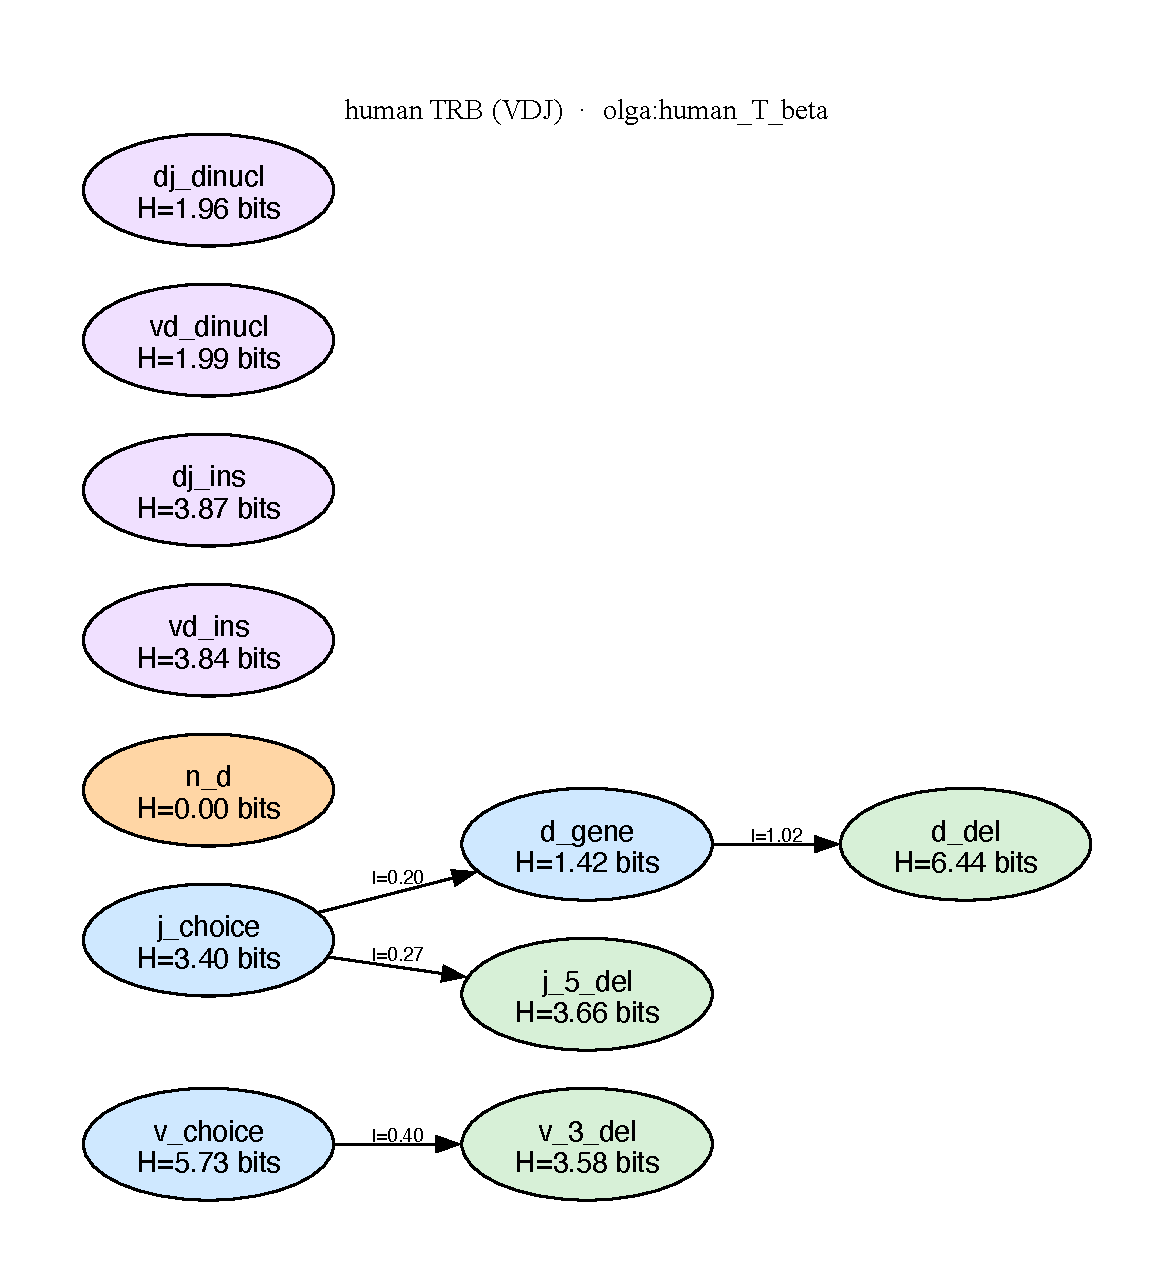
\includegraphics[width=0.49\linewidth]{bn_trb.pdf}\hfill
  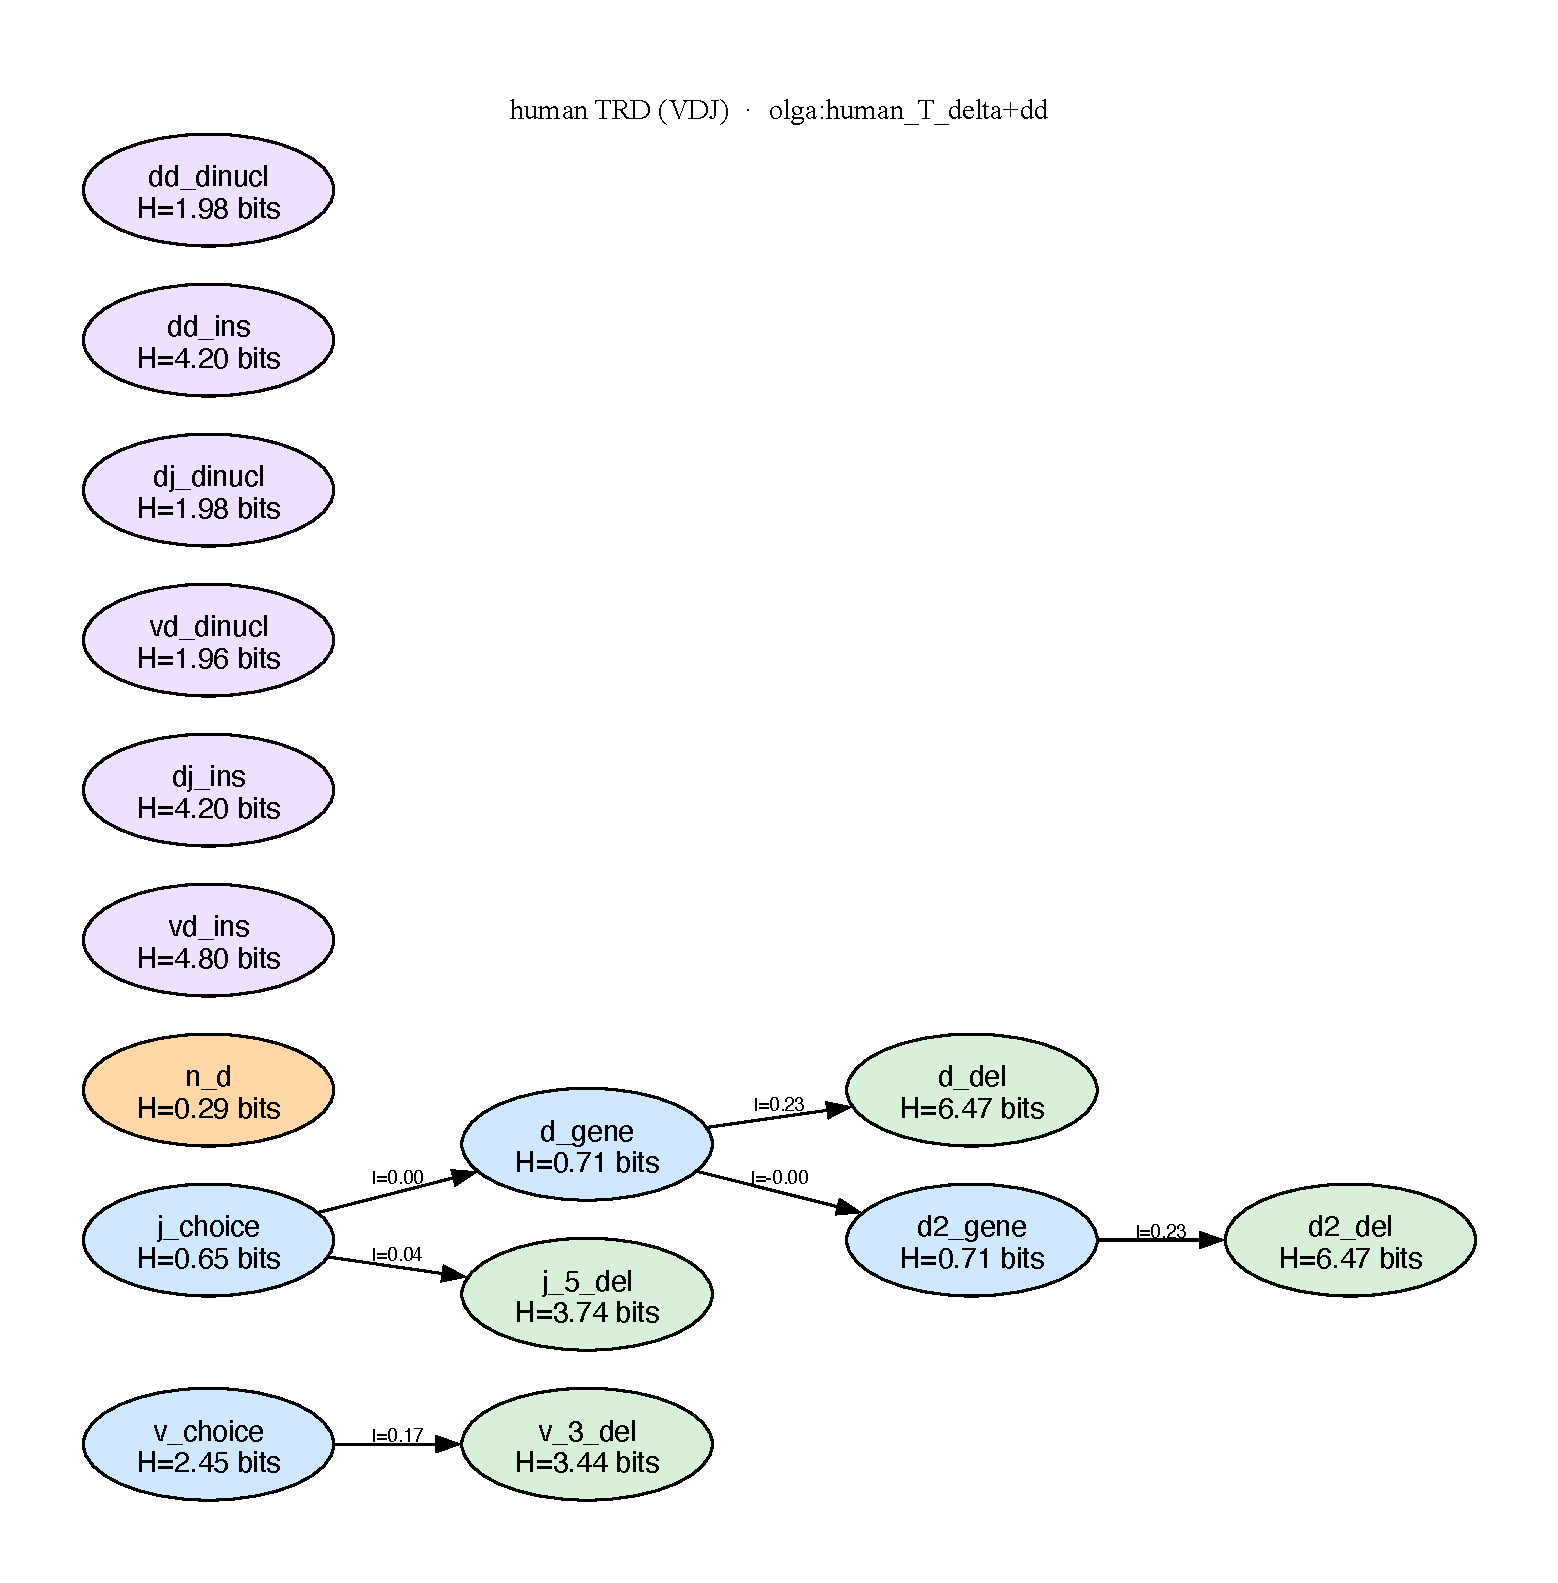
\includegraphics[width=0.49\linewidth]{bn_trd_dd.pdf}
  \caption{Historical recombination Bayesian networks rendered from frozen manifests, nodes labelled with marginal
    entropy $H$ (bits) and edges with mutual information $I$ (bits). \emph{Left:} human TRB (single-$D$).
    \emph{Right:} human TRD with the legacy tandem-$D$ representation, adding the $n_D$,
    $D_2$-gene, $D_2$-deletion and $DD$-insertion nodes. Current schema-3 fits
    replace the separate D-choice/count factors with $q_J(n,D_1,D_2)$ and
    separate branch-specific deletion tables (\S\ref{sec:dd}).}
  \label{fig:bn}
\end{figure}

Table~\ref{tab:entropy} retains a historical comparison of the per-event entropy across five frozen OLGA-reference loci; each row's most entropic
locus is in bold. Gene choice dominates in the $\alpha\beta$ loci ($H_V\!\approx\!5.7$
bits for TRB, $H_J\!\approx\!5.6$ for TRA), whereas TRD spends little on gene choice ($H_V\!=\!2.4$ bits,
few $\delta$ genes) and the most on non-templated insertion ($H_{VD}\!=\!4.8$ bits) --- the TdT signature.
The single most entropic event in every $VDJ$ locus is the joint $D$-deletion (up to $7.8$ bits for IGH),
and its two ends are far from independent: the within-$D$ coupling $I(\del_D^{5'};\del_D^{3'}\!\mid\!D)=1.18$
bits for TRB (a genuine conditional mutual information, averaged over $D$ so that the shared choice of $D$
does not inflate it). Two edges are worth naming. First, $I(V;J)=0$ for every $VDJ$ locus is not a
measurement but an \emph{assumption} made visible --- \texttt{OLGA} factors $P(V,J)=P(V)P(J)$ --- whereas
the $VJ$ loci carry $I(V;J)>0$ through $P(J\mid V)$ (e.g.\ $0.27$ bits for TRA). Second, the $D$-deletion
edge $I(\{\del_D\};D)$ is large
($1.02$ bits for TRB), i.e.\ trimming depends strongly on which $D$ was chosen. The identical routine
applies to an EM-inferred model, so the same table compares a model learned from real reads against the
\texttt{OLGA} bootstrap parameter-by-parameter. An earlier single-D, aligned-call-masked diagnostic on 6000 out-of-frame human
TRB clonotypes reported D-deletion entropy changing from $6.44$ to $7.65$ bits
and VD-insertion entropy from $3.84$ to $4.50$ bits, with within-D deletion
coupling near 1 bit under both fits.
Those values describe that diagnostic fit, not the current error-aware,
ambiguity-preserving isalgo models.
The producer's ``held-out'' label referred to its own training-report likelihood;
it did not constitute a held-out evaluation.
The independent functional-source validator in \texttt{compare\_models.py}
is described below and has a different purpose.

A separate historical annotation summary reported two aligned D segments in
4.15\% of out-of-frame and 3.42\% of in-frame unique human TRD clonotypes.
These are preliminary annotation fractions, not estimates of the current model's
posterior tandem frequency; the original summary did not record the denominators.


\begin{table}[t]
  \centering
  \small
  \caption{Marginal entropy $H(X)$ (bits) of each recombination event across five human loci, computed
    from frozen OLGA-reference model tables. These values are retained as
    historical diagnostics, not summaries of the current isalgo fits. Dashes mark events absent from a locus ($VJ$ loci have no $D$; $VDJ$ loci have no $VJ$ insertion). Bold marks the most entropic locus per event.}
  \label{tab:entropy}
  \begin{tabular}{lccccc}
    \toprule
    Event & TRB & TRA & TRD & IGH & IGK \\
    \midrule
    $V$ choice            & \textbf{5.73} & 5.37 & 2.45 & 5.71 & 4.81 \\
    $J$ choice            & 3.40 & \textbf{5.57} & 0.65 & 2.17 & 2.83 \\
    $D$ choice             & 1.42 & --- & 0.71 & \textbf{4.30} & --- \\
    $V\,3'$ deletion      & 3.58 & \textbf{3.69} & 3.44 & 3.46 & 3.15 \\
    $J\,5'$ deletion      & 3.66 & 3.89 & 3.74 & \textbf{4.13} & 3.65 \\
    $D$ deletion (5$'$,3$'$) & 6.44 & --- & 6.47 & \textbf{7.78} & --- \\
    $VD$ insertion length & 3.84 & --- & \textbf{4.80} & 4.68 & --- \\
    $DJ$ insertion length & 3.87 & --- & 4.20 & \textbf{4.82} & --- \\
    $VJ$ insertion length & --- & \textbf{3.84} & --- & --- & 3.59 \\
    $VD$ dinucleotide     & \textbf{1.99} & --- & 1.96 & 1.98 & --- \\
    $DJ$ dinucleotide     & 1.96 & --- & 1.98 & \textbf{1.99} & --- \\
    $VJ$ dinucleotide     & --- & \textbf{1.97} & --- & --- & 1.92 \\
    \bottomrule
  \end{tabular}
\end{table}

\FloatBarrier
\section{Implementation, validation and scope}\label{sec:implementation}

\paragraph{Code map} The Python reference scenario sums are in
\texttt{model/pgen.py}; packed native scoring and the transfer matrices are in
\texttt{src/pgen.cpp}, exposed by \texttt{model/native.py}.
\texttt{model/dd.py} declares and validates joint-history support;
\path{model/infer.py} owns proposals, EM updates and reports;
\texttt{model/data.py} owns the raw-data build.
\texttt{model/generate.py} provides reference/native sampling, and
\texttt{model/analyze.py} provides entropy and mutual-information summaries.
Paths beginning with \texttt{model/} are relative to \texttt{python/vdjtools/}.

\paragraph{Exactness and resources} The probability sums are exact over the selected
model support, apart from floating-point arithmetic; ``exact'' does not imply that
the reference includes every biological history.
Zero-mass branches are skipped algebraically without approximation.
The native single-D implementation shares short D-prefix states and reduces
right-boundary states within each query; these are transient DP workspaces.
With $S=25$ codon states, $d$ D templates, $T$ supported D deletion pairs per
template, maximum retained D length $G$, and insertion bounds $K_{VD},K_{DJ}$,
a conservative bridge bound is $O(dTNGS)$, in addition to germline seeding and
$O(NS(K_{VD}+dK_{DJ}))$ insertion recursions.
The single-D query workspace is $O(NS+NG)$ in addition to packed model tables.
Tandem scoring adds a J/D-pair traversal and a DD-insertion bridge; it is not
covered by a universal linear-in-length bound.
Native batch APIs share packed model state, release the GIL and bound their
query workers by the selected CPU allocation; \texttt{threads=0} uses that allocation.

\paragraph{Independent checks} \texttt{concordance.py} compares native nucleotide
and amino-acid scores to OLGA on the same legacy parameter family and checks
synonymous-codon sums when a sufficiently short generated query is available.
It is an engine check, not validation of an independently fitted model.
\texttt{compare\_models.py} separates this raw-reference oracle comparison from
software validation on freshly annotated functional-source reads outside the
nonfunctional training inputs.
Functional-source reads have undergone selection, so their likelihood is not an
unbiased held-out recombination objective.
The accepted validator selects the first 20000 raw reads and then the first
300 eligible unique junctions per context; the source bucket alone does not
prove every selected junction is productive.
For its OLGA oracle, three zero insertion bins extend the iteration workspace
without changing probability coefficients.
Focused tests cover joint-history normalisation, genomic constraints, allele
aliases, retained-germline errors and pruning, as well as the independent validator.
The historical timing and entropy tables above were not rerun for this revision.

\paragraph{Scope limits} The present engine supports the declared VJ, single-D and
up-to-two-D factorisations, not arbitrary Bayesian-network structures.
The observation channel covers retained-germline substitutions, not indels or
errors on inserted bases.
Candidate-gene restriction and positive inference cutoffs can remove compatible
histories; the latter reports actual omitted mass but does not bound it by the cutoff.
Gene-level reference selection does not infer an individual's allele genotype.
The entropy diagnostics describe the declared parameter support; dinucleotide
marginal entropies use stationary composition, and scenario-entropy contributions
weight first-base, transition and tandem events by their activation probabilities.
These summaries do not replace independent validation on matched references and inputs.

\clearpage
\bibliographystyle{unsrt}
\bibliography{refs}

\end{document}
